\documentclass[14pt]{beamer}
\usepackage{fontspec}
\usepackage{xunicode}

\usepackage{polyglossia}
\setmainlanguage{french}

\usetheme{Goettingen}
\useinnertheme{circles}
\beamertemplatenavigationsymbolsempty
\setbeamertemplate{footline}[frame number]

\usepackage{hyperref}
\usepackage{xkeyval}
\usepackage{xcolor}
\usepackage[timeinterval=5,timeduration=10]{tdclock}
\factorclockfont{3}

\renewcommand{\footnoterule}{}

\date{10 Juin 2014}
\author{Maxime \textsc{Gaudin} (\href{https://twitter.com/maxigaud}{@maxigaud})}
\title[{\cronominutes:\cronoseconds}]{Un hackathon ?\\ Pourquoi faire ?}

\begin{document}
\begin{frame}
	\titlepage
	\initclock
\end{frame}

\begin{frame}{FHacktory 2014}
	\begin{center}
		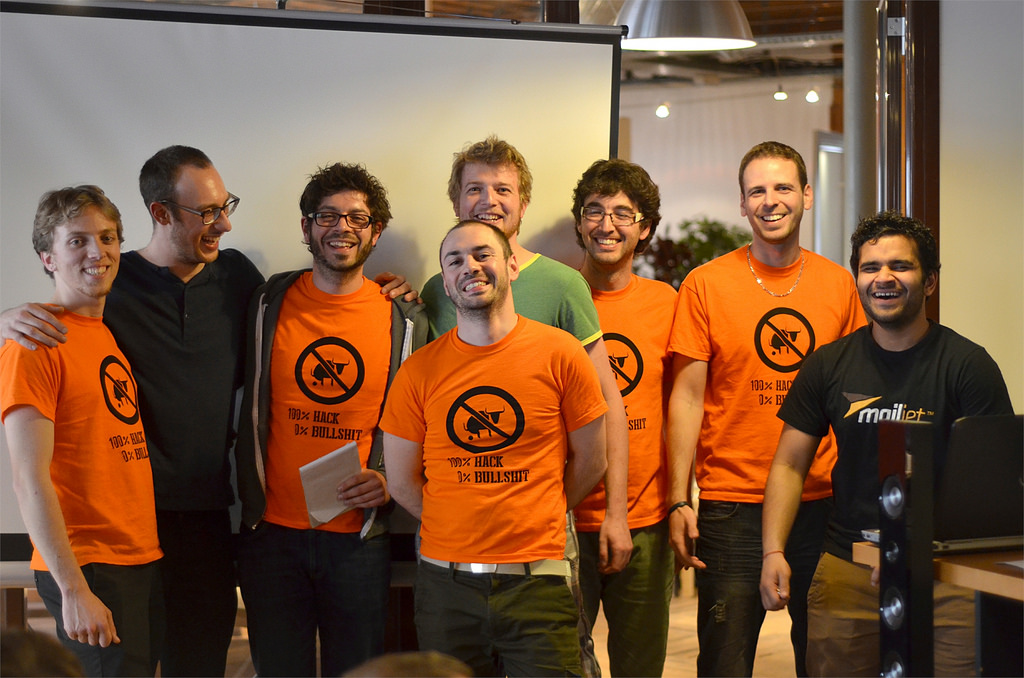
\includegraphics[width=\textwidth]{img/win_picture}
	\end{center}
\end{frame}

\begin{frame}{Notre projet}
		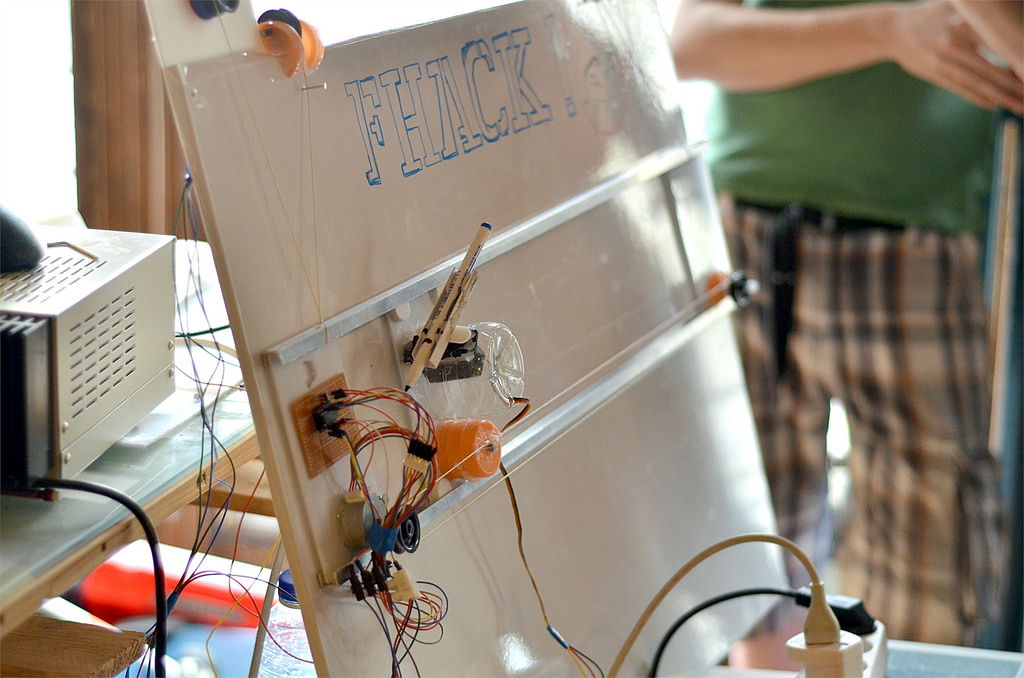
\includegraphics[width=\textwidth]{img/Veledrawbot}
\end{frame}

\begin{frame}{Pourquoi ne {\bf pas} faire un {\sl hackathon}}
	\begin{itemize}
		\item Pour gagner
		\item 	Pour la gloire
	\end{itemize}
\end{frame}

\begin{frame}{Pourquoi faire un {\sl hackathon} ?}
	\begin{itemize}
		\item Pour se retrouver
		\pause\item Pour rencontrer 
		\pause\item Pour s'amuser
		\pause\item Pour apprendre (une méthode plus qu'une technique)
		\pause\item Pour créer son MVP\footnote<5->{\sl Minimum Viable Product} et tester son idée
	\end{itemize}
\end{frame}

\begin{frame}{Quelques conseils}
	\begin{itemize}
		\item Préparation
		\pause\item Lâcher prise
		\pause\item {\bf Sommeil}
		\pause\item Pistolet à colle
		\pause\item Préparation
	\end{itemize}
\end{frame}

\begin{frame}{Merci}
	\begin{exampleblock}{Des questions ?}
	\end{exampleblock}
\end{frame}

\end{document}{beamer}